\chapter{On Nesting Graphs}\label{cha:nesting}

\epigraph{\textit{Did she say: ``He yelled, \lq Frame stories are an example of nestings in literature!\rq\;''?}.}{--- An example of a nested quote.}

\newcommand{\trf}{\hl{\texttt{[REF]}}}
Graph data management systems play an increasing role in present data analytics, because they allow flexible analyses of relationships among data objects. In fact, graphs have been already used as a fundamental data structure for representing data within different contexts (corporate data \cite{success,Park2016355}, social networks \cite{xie,BrodkaK14}, statistical correlations \cite{StatisticalModels} and linked data \cite{Vasilyeva13,BarabucciEARMARK}). Despite the increasing production of graph data, a general operator aggregating with a roll-up fashion one single graph is missing. This operator should create \textbf{nested vertices} and \textbf{nested edges}, which may contain other graphs; we would also like that those components may be freely unnested. The edges connecting the nested vertices do not necessarily represent a partition of the input graph, but the presence of an edge between two summarized vertices represents the existence (within the input graph) of an edge (or more generally a path) between the partitions which the aforementioned vertices represent. Therefore, such desired outcome extends the \textit{vertex summarization} class of aggregations: those strategies prefer to group the vertices as in relational \texttt{Group By} strategies, and then aggregate the edges accordingly \cite{JunghannsPR17}. These class of operations restrict the ability of aggregating by paths, that are limited to the set of edges connecting the vertices belonging to two (different) class of vertices. It follows that such class of aggregations   do not allow to freely aggregate the edges into final nested edges. 


\begin{figure}[!t]
	\centering
	\begin{minipage}[!t]{0.6\textwidth}
		\centering
		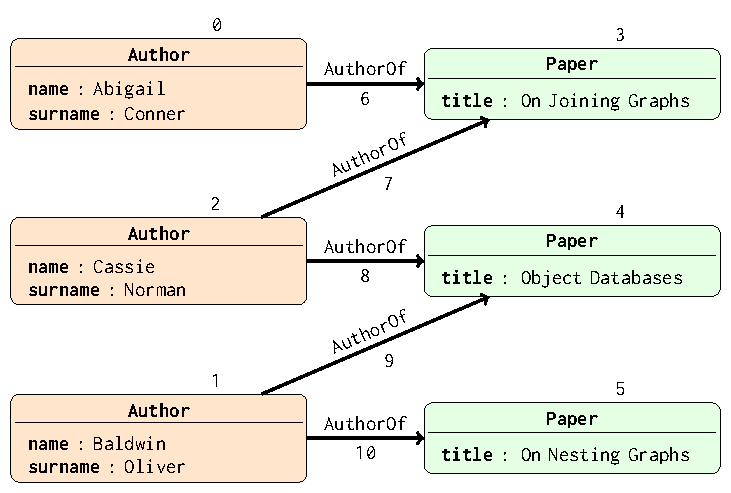
\includegraphics[width=1\textwidth]{imgs/03introduction/04bibliography}
		\subcaption{Input bibliographical network.}
		\label{fig:inputbibex2}
	\end{minipage}
\medskip

	\begin{minipage}[!t]{\textwidth}
		\centering
		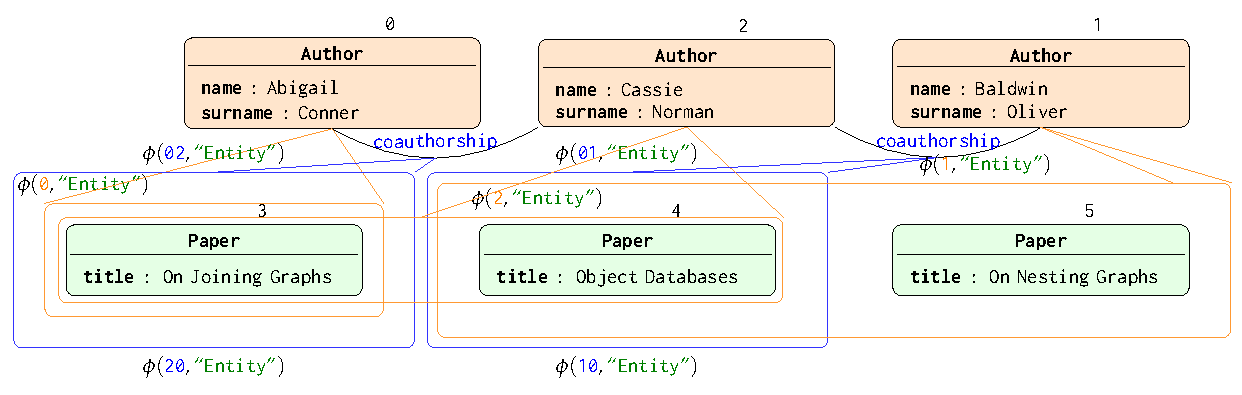
\includegraphics[width=\textwidth]{imgs/03introduction/042nested}
		\subcaption{Nested result: given two \texttt{Author}s $\color{orange}a$ and $\color{orange}a'$, there exist two  \texttt{coauthorship} edges, $\color{blue}a\to a'$ and $\color{blue}a'\to a$ if and only if they share some authored paper contained respectively in $\phi({\color{blue}a\to a'},\ONTA)$ and $\phi({\color{blue}a'\to a},\ONTA)$. Moreover, each author $\color{orange}a$ is associated to the set of his authored papers $\phi({\color{orange}a},\ONTA)$. }
		\label{fig:outputnested}
	\end{minipage}
	\caption{Nesting a bibliographic network. While in the previous Example \vref{ex:bigraphbibnet} the information was summarized, in this case the provenance information is nested within the original node. }
	\label{fig:bibex2}
\end{figure}
Since most of such vertex summarization techniques are graph-partition based, most of them fail to aggregate graphs that share some vertices and edges in common: as we have already seen in both Section \vref{sec:informationsintegration} and \vref{subsec:nested-partof}, social networks often contain communities which users may overlap and, when aggregating a social network on top of such communities, we need to be able to perform such aggregations even on this situation. Among all those graph summarization techniques, only HEIDS \cite{ChengJQ16} and Graph Cubes \cite{Zhao11} perform graph summarizations of one single graph over a graph collection of non pairwise disjoint subgraphs. On the other hand, these last two techniques require that the set union of such graph collections must be equivalent to the original graph, while data integration and social networks scenarios even consider the possibility of outliers within the data, that are hereby represented in no subgraph belonging to the aforementioned graph collection. %To overcome to this graph operation limitation, this thesis proposes the \textbf{graph nesting} operator, thus providing a general graph summarization technique.
Such approaches were not compared to already existing (graph) query languages and, consequently, we provide a general graph nesting definition in Section \vref{def:graphnesting} and its generic implementation in Section \vref{subsec:polyovergraph} as the first naïve (but general) algorithm for a graph nesting. Such straightforward implementation  proves to be inefficient, because the visit of such graph collections of size $k$ (to be nested within the graph operand) implies to perform, in the worst case scenario, $|g|^k$ visits of the graph operand $g$: this results into an exponential algorithm, because the size of $k$ may vary, while $|g|$ is fixed. This implies that the graph must be always visited more than once, even if this may not be required. Even though this general operator proves to be inefficient in practice, it allows to detect a broader class of problems and of optimizable algorithms.

In order to reduce the graph visiting cost from $|g|^k$ to $O(|g|)$, we could use a graph traversal approach: instead of pre-computing $k$ subgraphs of $g$ that are going to be later on used to nest $g$, we can directly perform the graph nesting while visiting the graph, thus allowing  not to perform additional costs for comparing the resulting graphs in a later step. The following example shows how such queries can be efficiently formulated and implemented.

\begin{example}
	\label{ex:nestingbib}
	We're going to consider the same bibliographic network summarization problem presented in former Example \vref{ex:bigraphbibnet} and Section \vref{sec:semistructunstradata}: given a bibliographic network containing (at least) \textsc{Author}s and \textsc{Paper}s as vertices, and where \textsc{authorOf} edges connect each author to the papers he has authored (Figure \ref{fig:inputbibex2}), ``project'' the network into a coauthorship network, where each \textsc{Author} is connected by a \textsc{coAuthor} edge with another  \textsc{Author} with which he has published some paper (Figure \ref{fig:outputnested}). In particular, for each resulting \textsc{Author} vertex nest inside it all of its papers as vertices, and nest inside each \textsc{coAuthor} edge all the papers coauthored by both the source and destination \textsc{Author}s. Exclude \textsc{coAuthor} hooks over the same vertex.
	
	This problem can be solved by visiting the graph starting from the vertices: if the current vertex is a \textsc{Paper}, traverse backwards all the \textsc{authorOf} edges, thus reaching all of its \textsc{Author}s, that are going to be \textsc{coAuthor} for at least the current paper. Therefore, I can incrementally define the edge nesting between all such authors in a separated nesting index, since I know that all these authors share the same paper, and partially instantiate the nesting of each author with the papers that has authored via an external index. All the other vertices and edges may be discarded as a starting point for the graph visiting process. By doing this, only the edges are visited twice, but the vertices are visited only once. Hereby, with these patterns we reach the optimal solution by visiting the graph only once.
\end{example}

The usage of graph traversal approaches for graph nesting allows \textit{path summarizations} as well as vertex summarizations: path summarizations (described in more detail in Section \vref{subsec:pathsumm}) allow the aggregation of multiple paths together among source and target vertices that share the same property. The problem with both path and vertex summarizations is that no general class of either source and target vertices can be used as an outcome of a previous community detection \cite{xie,berlingerio11} or data cleaning and alignment phase \cite{ALIEH17} without rewriting the previously extracted data into an explicit query, thus requiring an additional pre-processing step and thus making such approach not as flexible as required by data integration scenarios. %initial query each time after different vertex data is extracted, thus not allowing to use such query definition for general data integration scenarios. 
 This problem is also reflected by pattern matching query languages, where the vertex summarization phase must be necessarily separated from the path summarization one, thus thwarting the advantages of performing vertex and path summarizations contemporarily. In particular, while Cypher queries can perform distinct aggregations only within distinct \texttt{MATCH} clauses, SPARQL 1.1 implementations of the query plan combine these two phases with a \texttt{UNION} operator, thus forcing the algorithm to visit the same graph twice. As a result, the query plan optimizers of such query languages do not allow to avoid to visit one same graph more than once whether possible.  

This chapter shows that such limitations can be reduced by using a graph nesting operator, which embodies both vertex and path summarization queries, which are performed contemporarily within the same operator. %The following example provides an example of how such query can be formulated and performed. --> Old example
We also investigate a data structure and a general algorithm to optimize graph nesting operations. To that end, we study the existence of specific graph patterns prone to algorithmic optimizations, similar to relational $\theta$-join algorithms over specific $\theta$ predicates (Section \ref{sec:optimizableClass}). Hereby, we show that such algorithmic approaches allow to reduce the time complexity of the visiting and nesting problem, which is going to performed over a data structure that requires less indexing time that its own competitors. In particular, we focus on intersecting graph visiting patterns: one pattern ($g_V$) is given for vertex summarization, and the other ($g_E$) is for path summarization into one single edge, thus subsuming which is the shared sub-pattern ($\alpha$) among the two former ones. Consequently, $\alpha$ is going to be visited only once within the graph, after which either the vertex or the path summarization pattern can be visited in their entirety. We also perform some restrictions over these patterns enhancing such optimizations: for each vertex pattern we're going to elect one vertex called \textbf{vertex grouping reference} ($\gamma_V$), over which we're going to nest the elements matched by the graph pattern met during the visit. Similarly, each edge path summarization pattern is going to elect a source ($\gamma_E^{src}$) and a target ($\gamma_E^{dst}$) vertex, which are going to be called \textbf{edge grouping references}: such vertces must both coincide with the vertex grouping references, so that the newly generated edge will have as sources and target the previously vertex-nested elements. 


\begin{figure}[!t]
	\centering
	\begin{minipage}[!t]{0.5\textwidth}
		\centering
		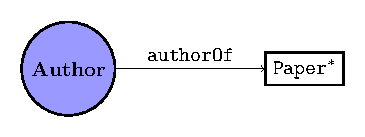
\includegraphics[width=.7\textwidth]{images/nesting/patterns/00_vertex_pattern.pdf}
		\subcaption{Vertex summarization pattern.}
		\label{fig:vertexPat}
	\end{minipage} \begin{minipage}[!t]{0.5\textwidth}
		\centering
		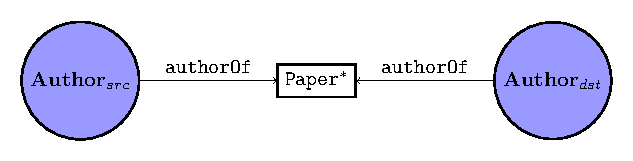
\includegraphics[width=1\textwidth]{images/nesting/patterns/00_path_pattern.pdf}
		\subcaption{Path summarization pattern.}
		\label{fig:pathPat}
	\end{minipage}
	\caption{Vertex and Path summarization patterns for the query expressed in Example \vref{ex:nestingbib}. Vertex and edge grouping references are marked by a light blue circled node. As we can see, the vertex grouping reference depicts the same property expressed by edge grouping references.}
	\label{fig:patterns}
\end{figure}
\begin{example}[continues=ex:nestingbib]
Figure \vref{fig:patterns} represents the desired vertex and path summarization patterns. As we can see, the same vertex summarization pattern appears twice within the path summarization: this means that by visiting the path summarization pattern once, we may pre-istantiate two morphisms for the vertex summarization pattern. The two patterns have different key roles: while the vertex summarization retrieves all the papers that one author has published and nest them within one single matched author, the path summarization return all the papers authors by two different authors and creates an edge between the two previously nested vertices. This construction implies that a join between the two paths must be carried out. 

This pattern comparison remarks that, in order to reduce the graph time visit, we must start from visiting the \texttt{Paper}, which is shared among the two distinct patterns, and then keep going with the graph visit by exploring the source and target vertices. 
\end{example}

There might be other possible patterns that can be optimized, but we're going to focus just on vertex and path summarization patterns where edge grouping references are connected to each other at a 2 edge step distance (Section \ref{sec:THOSPA}). We're also going to show how such optimizations can be detected beforehand by looking at the pattern representation.


Last, we implemented the aforementioned solution into a nested graph data model, which directly extends the graph data model used for graph joins in Chapter \vref{cha:join}. We performed our benchmarks on both relational models supporting JSON (PostgreSQL), RDF (Virtuoso) and Property Graph (Neo4J) stores, and document based databases supporting graphs (ArangoDB). The results of such experiments shows that the sum of both indexing and query evaluation time of our proposed solution outperforms by at least one order of magnitude the aforementioned solutions evaluated on such databases with their respective query languages (Section \ref{sec:nestexpeval}). Consequently, our data model also proved to be curcial in providing an enhanced implementation of the specific nesting algorithm. 

This chapter provides the following main contributions:

\begin{itemize}
	\item \textbf{Graph Nesting Operator} (Section \ref{sec:nestingdef}); we provide a general definition of the nesting operator which combines the path  with the vertex summarization approaches to nesting graphs.
	\item \textsc{{Two HOp Separated Patterns}} \textbf{(THoSP) algorithm for a specific graph nesting task} (Section \ref{sec:THOSPA}): we
	compare it to its implementation
	over both graph  (SPARQL, Cypher), relational (SQL) and document oriented (AQL) query languages: as a result our solution outperforms
	the query plan implementation of the other query languages and scales on the large.
	\item A general strategy on how to extend the THoSP algorithm for patterns having vertex and edge grouping references is provided (Section \ref{sec:optimizableClass}).
	%\item By extending the concept of binary predicates into edges, Edge Joins are introduced as a preliminary step towards the definition of Graph Nesting (Chapter \vref{cha:nesting}).
\end{itemize}


%Even though the previously defined graph join operator provides a binary operator for combining two distinct data sources into one single representation, such operation is not general enough for providing proper graph data integration: such operation only performs a binary aggregation over the vertices matching in the two data sources, it is not possible to aggregate more of one vertex per operand into one single aggregated vertex (Section \vref{sec:whynotjoins}). 

%This solution can be also attacked by using current \textbf{graph summarization} operations \cite{biafore}:
%current graph query languages can perform graph summarizations along paths (\textbf{path summarization}), while some others focused more on summarizing graphs on their vertices (\textbf{vertex summarization}). Instead of performing graph joins, we can consequently  perform the set union of all the incoming graph data sources and then aggregate the resulting graphs using the aforementioned operations. 

%For subsequent operation on such summarized graphs, it is desirable that information about contained vertices and edges of these new elements is preserved, for example, to ensure provenance or to support OLAP operations such as drill-down. Existing approaches, such as ($k$-)SNAP \cite{Tian20085} and I/T Aggregations \cite{chenyzhy08,Qu2011}, create new graphs to represent summaries and must use external indexing structures for backtracking to the previous non-aggregated data. However, a data model optimally should bear the original information within the summarized vertices to make them accessible when required, and should allow to drill-down to other graph representations that do not necessarily include previous aggregated stages. As we already seen in the previous chapters, the Nested Graph definition allows to meet all such requirements (Definition \vref{def:NestedGraphModelThesis}), and hence it is chosen as the default data representation within this paper.

%The \textit{path summarization} 






%% Opening
% * What is the wider problem that we should try to solve?
% * Say that this is an already known problem
% A valuable class of analytical graph operations are these creating new vertices and edges from existing graph elements. Such operations include \textit{graph grammars} \cite{ModCheckWithGG,Eichler2016,Rozenberg,GraphLogAggr}, \textit{vertex fusions} \cite{petermann2014biiig} and \textit{graph grouping}. First, \textit{graph grammars} replace a pattern describing authorships in a bibliographic network using dedicate edges among authors. Secondly, in the process of graph-based data integration scenario, \textit{vertex fusion}s can fuse a subgraph of vertices representing the same logical entity into a single vertex. 
 
 %%%%%In order to find more general approaches, one must analyse the \textbf{graph summarization} approaches that have been designed for graph-based MOLAP scenarios. These approaches allow to analyze and to visualize large graphs \cite{ChengJQ16}, mapping each graph partition into one single vertex or edge. 
 %%%


%To overcome this data representation problem, we propose a novel \textit{nested property graph model} (NPGM). Current property graphs are one of the most popular models of well established graph data management systems. In this model each vertex and edge bears its own attributes, values and labels. To support element nesting, we extend the model by associating a \textit{structural content} to every vertex and edge, or \textit{content} in brief.
% , and vertices (and edges) with both empty and non empty nestings coexist. 


%\input{101_figures}

%% Background
% * Which informations must the reader know in order to
%   understand the problem?
%Basically, an element's content is a (possibly empty) set of vertices' and edges' identifiers. Moreover, our model allows different vertices and edges to (partially) share their content with other vertices and edges. This scenario appears, for example, when summarizing a social network, like the one provided in Figure \ref{fig:osn}. Such summaries can help to reveal community interactions at a broader level. A natural representation of communities in social network are subgraphs of users and their friendships. Therefore, every community can be represented by a \textit{nested vertex} and the original users as well as their relationships are the content (e.g., vertices $7$ and $8$). Further on, friendships among users of distinct communities can be aggregated and represented by \textit{nested edges} (e.g., edges \textit{viii}, \textit{ix} and \textit{x}). However, a distinct user may belong to different communities, i.e., is content of multiple nested vertices (e.g., vertex $5$ for vertices $7$ and $8$). Our model allows to query such overlaps and to reflect their existence by establishing dedicated edges. 
% \subsubsection*{(How does the challenge contributes to the opening, which is
%% wider than our aim?)}
% The present data model also allows to reduce the number of the operators to be used for graph analytics processes: within the previous graph data models model, graphs and graph collections were two different data types \cite{Ghrab2015, junghannsdistributed}, and hence we had to distinguish the operators returning a graph from the ones returning a collection of graphs. As  a consequence, operations like union, intersection and difference had to be re-defined for the two data classes. Since now the present data model allows complex vertices to contain other complex vertices, each vertex could represent either a graph or a graph collection. Therefore, the aforementioned operations collapse into just one operation over nested graphs and nested graphs are closed under the set of operations to be defined on top of this data model. 
% \medskip
%Although the development of the nested property graph model is work in progress, this short paper contains the following contributions:

%\begin{itemize}
 % \item We propose an extension to the popular property graph model to support nested vertices and edges (Section \ref{sec:datamodel}).
  %\item We present a generalized operator that can be configured to support different operations such as graph transformation or graph summarization  (Section \ref{sec:nestedOp}).
  %\item We discuss the requirements of graph pattern matching languages for nested property graphs (Section \ref{sec:patternmatching}).
%\end{itemize}
%Additionally, we discuss our model in comparison to existing graph data models in Section \ref{sec:related} and draw some conclusions in Section \ref{sec:concl}. 
